\chapter{Introduction}
\label{introduction}

\section{Problem Statement}
\subsection{Voronoi Diagram}
Voronoi diagram is a special kind of decomposition of a space, determined by distances to a given set of objects in the space. As a fundamental geometric data structure, Voronoi diagrams have been widely applied in various computer graphics and visualization applications, including collision detection~\cite{Sud:2006:FPC:1141911.1142006},
meshing~\cite{DBLP:journals/cgf/YanLLSW09}, vector field visualization~\cite{DBLP:conf/vissym/McKenzieLD05}, artistic effect, image %~\cite{Dobashi_Haga_Johan_Nishita_2002}%
segmentation~\cite{DBLP:journals/tip/WangJW11}, just to name a few. Among many efficient algorithms for construction of Voronoi diagram,Fortune's sweep line algorithm~\cite{Fortune1986} is popular due to its elegancy and simplicity. Given a set of 2D points (called \textit{sites}), the sweep line algorithm maintains a vertical sweep line moving from left to right across the plane as the algorithm progresses. At any time during the algorithm, the input sites on the
left side of the sweep line have already been incorporated into the Voronoi diagram, while the sites right of the sweep line have not been considered yet. Each site to the left of the sweep line generates a parabola of points equidistant from that point and from the sweep line. The wavefronts of all parabolas form a curved beach line, which follows the sweep line moving from left to right. As the sweep line progresses, the vertices of the beach line, at which two parabolas cross, trace out the edges of the Voronoi diagram. The sweep line algorithm is proven to be optimal with $O(n\log n)$ time complexity and $O(n)$ space complexity.

In spite of its simplicity and popularity, there is no effective technique to parallelize the sweep line algorithm.Thurston~\cite{Thurston:1986} pointed out that if the input vertex set is very large, then the sweepcircle technique allows one to compute the Voronoi diagram locally~\cite{Klein:1988:VDB:646504.696442}. Dehne and
Klein~\cite{Dehne_Klein:1987} proposed a {\em sweepcircle} technique to compute the \textit{transformed} Voronoi diagram, where the transformation is made in polar coordinates:
\begin{equation}\label{eq:transformation}
\vspace{-2mm}
    x\triangleq(\rho,\theta)\longrightarrow x'\triangleq(\rho+|x-x_i|,\theta),
    \vspace{-2mm}
\end{equation}
where $x_i$ is the nearest site to $x$. The purpose of this transformation is to guarantee that the site $s$ is touched before the Voronoi cell of $s$ is swept by a sweeping circle. They proved that the transformed diagram has the same combinatorial structure as the original Voronoi diagram~\cite{Dehne_Klein:1987}. This
transformed sweepcircle algorithm is parallel in nature and can be also applied to compute the Voronoi diagram on cones. However, it is difficult to represent the transformed Voronoi edges from the implementation perspective, since they are not straight line segments or conic curves anymore. To our knowledge, there is no
practical implementation of the sweepcircle algorithm.


\subsection{Centroidal Voronoi Diagram}
A centroidal Voronoi tessellation (CVT) is a particular
Voronoi tessellation of a compact domain in Euclidean space
yielded by a set of samples such that each site locate at the same place with the centroid of its Voronoi cell. For example, Figure\ref{fig:voronoi_and_CVT_2D}(a) shows
a Voronoi tessellation of a circular domain where the sites
do not locate at the same place with the centroids of the Voronoi cells (not a CVT),
 while Figure\ref{fig:voronoi_and_CVT_2D}(b) shows a CVT of the same domain. CVT generates
an evenly spaced distribution of sites in the domain with respect
to a given density function, and is therefore very useful in many
fields, such as optimal quantization, clustering, data compression,
optimal mesh generation, cellular biology, optimal quadrature, coverage
control, and geographical optimization. An excellent introduction
to the theory and applications of CVT is given in Du et al.~\cite{Du:1999:CVT}
 and Okabe et al.~\cite{Okabe:2000}.

\begin{figure}
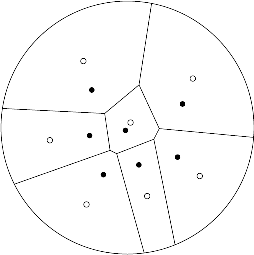
\includegraphics[width=3in]{figs/intro/voronoi_2D.png}
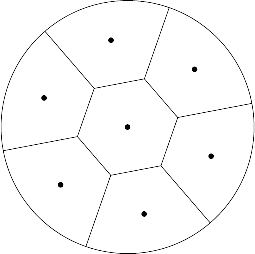
\includegraphics[width=3in]{figs/intro/CVT_2D.png}
\caption{(a) An ordinaryVoronoi tessellation of a circular domain with seven sites marked with black dots and the the centroids of the Voronoi cells marked with small circles; (b) a CVT of the same domain with seven sites.Anisotropy sampling is useful in many geometry applications, such as object distribution, vector field visualization. Figures are taken from ~\cite{Liu:2009:CVT}  }
\label{fig:voronoi_and_CVT_2D}
\end{figure}

CVT has recently been applied to the surface remeshing problem. Surface meshing is a fundamental problem due to the dominance of triangle meshes in computer graphics and visualization. The past decade has witnessed significant progress in surface meshing. Among many promising techniques, the centroidal Voronoi tessellation (CVT) has received much attention recently. CVT is a special kind of Voronoi diagram (VD) in which the generating point of every Voronoi cell is also its center of mass~\cite{Du:1999:CVT}.

Most of the existing CVT techniques focus on the numerical solver of
the CVT energy function. The Lloyd algorithm ~\cite{Lloyd:1982} iteratively
moves the generator of Voronoi cell to its mass center. Although
being conceptually simple and easy to implement, the Lloyd algorithm
has only linear convergence rate. Liu et al. ~\cite{Liu:2009:CVT} proved that the energy function of CVT is $C^2$ continuous in general. As a result, we
can minimize the CVT energy by the Newton or quasi-Newton solver,
which converges much faster than Lloyd algorithm. However, both
solvers require computing the Voronoi diagrams in each iteration. It
is fairly simple to construct the Voronoi diagrams in Euclidean
space (e.g. $\mathbb{R}^2$ and $\mathbb{R}^3$), since many efficient
algorithms and software tools are readily available. However, it is
technically challenging to compute VD on curved surfaces. Therefore,
some researchers tackle this challenge by computing the restricted
Voronoi diagrams~\cite{Yan:2009:IRF:1735603.1735629}, which is the
intersection between a 3D Voronoi diagram and an input triangle mesh.
These approaches are embedding space dependent and may fail for
models with complicated geometry. Others rely on the global
parameterization, where the input surface is parameterized to the
Euclidean plane $\mathbb{E}^2$, sphere $\mathbb{S}^2$, or hyperbolic
disk $\mathbb{H}^{2}$. Then the 2-dimensional CVT is computed in the
parametric domain, which induces a meshing on the input triangle mesh. It
is known that the global parameterization is computational high cost
and may cause some numerical issue if the parameterization has large
distortion.


\section{Objectives}

This report aims to find a fully parallel sweep-circle algorithm for calculating a Voronoi Diagram,and a parallel and intrinsic algorithm for generating CVT on a surface.

\subsection{Fast Parallel Algorithm for a Voronoi Diagram}

This report aims to tackle the challenge of fast computing a Voronoi Diagram by proposing a new algorithm, called the {\em untransformed
sweep-circle}, for computing a 2D Voronoi diagram. Starting with a
degenerate circle (of zero radius) centered on an arbitrary point
(not necessarily a site), as the name suggests, our algorithm sweeps
the circle by increasing its radius across the plane. At any time
during the sweeping process, each site inside the sweep-circle
defines an ellipse composed of points equidistant from that point
and from the sweep-circle. The union of all ellipses forms the beach
curve, a star shape inside the sweep-circle which divides the
portion of the plane within which the Voronoi diagram can be
completely determined, regardless of what other points might be
outside of the sweep-circle. As the sweep-circle progresses, the
intersection of expanding ellipses traces out the Voronoi edges.

We show that the sweep-line algorithm is a degenerate form of the
proposed sweep-circle when the circle center is at infinity, and our
algorithm also has the same time and space complexity as its line
counterpart. However, our algorithm fundamentally distinguishes
itself from the sweep-line algorithm in that it allows multiple
circles at arbitrary locations to sweep the domain simultaneously.
This leads to a very natural parallel implementation,
while the sweep-line algorithm does not have such a feature. Compared with the traditional sweep-circle technique~\cite{Dehne_Klein:1987},
our algorithm is fairly easy to implement, since the most complicated numerical operation is nothing more than an arc cosine calculation.
Furthermore, our algorithm supports the computation of additively
weighted Voronoi diagrams in which the Voronoi edges are hyperbolic and
straight line segments.


\subsection{Centroid Voronoi Diagram on a Surface, and Remeshing}

This report presents a fully intrinsic and parallel algorithm for
calculating CVT on a surface.

This report falls into the category of CVT-based meshing. Instead of
using global parameterization or relying on the embedding space,
we propose a new algorithm to calculate the CVT on surfaces
directly. Our key idea is to use exact geodesic distance to calculate intrinsic CVT.
It is worth noting that our method is independent of the embedding space and fully intrinsic.
We propose an effective algorithm to compute the approximate CVT on arbitrary surfaces. Compared to the conventional CVT techniques, our algorithm is computationally efficient, conceptually simple, and easy to
implement.

Based on our new CVT algorithm, we develop a computational
framework to generate high quality isotropic and adaptive triangle
meshes. Compared to the existing meshing techniques, our method is
completely intrinsic and insensitive to the resolution/tessellation
of the input surfaces. We demonstrate the efficacy of our method in
a variety of real-world models. Thanks to its intrinsic nature,
our method works well for models with arbitrary topology and
complicated geometry, where the existing extrinsic approaches often
fail.

Meshes are an important way to represent shapes. A large number
of these meshes are generated by scanning devices, isosurfacing implicit representations or modeling software. These meshes often lack
the properties desired for subsequent geometric processing. For example,
a poor triangulation may result in the failure of some numerical
methods. Therefore, surface remeshing has been extensively studied
in the past 20 years. The readers can refer
\cite{Heckbert_Garland:2004,Talton:2004,alliez-remeshing-survey:2008}
for a complete survey.

Surface remeshing may have various purposes, depending on the type of application in which it is used.
For instance, structured meshes offer a simpler connectivity graph,
thus allowing for efficient localization and traversal
in the algorithms. In this report, we aim at proposing a high-quality remeshing algorithm,
i.e., approximating the model geometry with a high-quality triangle mesh
while preserving geometric features. We are aware that,
Liu et al.~\cite{Liu:2009:CVT} proposed an elegant method
for this purpose. They found that by considering
Centroid Voronoi Tesselation~(CVT) in the embedding space,
it is possible to obtain a group of uniformly distributed seed points
that define a high-quality triangle mesh. However,
Rong et al.~\cite{Rong:2011:CVT} pointed out that their algorithm
is not intrinsic and therefore cannot deal with models with narrow
and flat parts or in higher dimensional space.

Observing that a discrete exponential map~\cite{Schmidt:2006} can
bridge the gap between 2D CVT and uniform point distribution on
2-manifolds, we propose a new framework for surface remeshing.
Initially, we get a collection of random distributed sample points.
Then in a parallel style, we locally map the
seed points onto the tangent plane by discrete exponential mapping
, calculate their centroid in 2D,then map the centroid back to the surface.
We repeat this process until the energy magnitude is within a prescribed tolerance.
Finally, we extract the re-triangled mesh conforming to the geodesic
Delaunay triangulation. By encoding the geometric feature
information into a density function, our framework can easily
support an adaptive distribution of seed points. Compared with
existing remeshing algorithms, our algorithm is parametrization
 free, adaptive, intrinsic, parallel in nature and insensitive to the
original triangle quality.
\section{Thesis Organization}

In the following report, we first review the related work on conformal parametrization for computer graphics in Chapter \ref{chap:RelatedWorks}, then we introduce the mathematical background for conformal map in Chapter \ref{chap:background}. In Chapter \ref{chap:theorem} we will discuss our work to compute extremal quasi-conformal map on general surface.
Chapter \ref{chap:brainstem} presents the work by using ricci flow and extremal quasi-conformal map to build the surface registration on brainstem for the study of AIS, in addition in Chapter \ref{chap:vs} we use the holomorphic 1-form and extremal quasi-conformal map to build the registration of the vestibular system.
In Chapter \ref{chap:grip}, we propose a solution for 2D/3D sensor network greedy routing by applying a parametrization similar to the conformal map to build the
virtual coordinate system first. In Chapter \ref{chap:droste}, we use the conformal map as a basic image editing tool to generalize the traditional Escher-Droste effect.
Lastly, we conclude our work and provide some future directions for conformal maps in Chapter \ref{chap:conclusion}.
